\section{The Riemann Integral}

\begin{definition}
Let $I = [a, b]$, where $a$ and $b$ are real numbers, be a subset of $\mathbb{R}$ and let 
\begin{align*}
    P = \{x_{0}, x_{1}, x_{2}, ..., x_{n-1}, x_{n}\} \hspace{20pt} \text{such that} \hspace{20pt} a = x_{0} < x_{1} < x_{2} < \cdots < x_{n-1} < x_{n} = b
\end{align*}
be a finite subset of numbers contained in $I$. Take each of member $x_{i}$ of $P$ and use it to create a sub-interval $I_{i}$ of $I$, such that the union of these sub-intervals is $I$, as follows
\begin{align*}
    I_{0} = [x_{0}, x_{1}) \hspace{20pt} I_{1} = [x_{1}, x_{2})& \hspace{20pt} \cdots \hspace{20pt} I_{n-2} = [x_{n-2}, x_{n-1}) \hspace{20pt} I_{n-1} = [x_{n-1}, x_{n}]\\[2ex]
    &I = I_{0} \cup I_{1} \cup I_{2} \cup \cdots \cup I_{n-1} \cup I_{n}
\end{align*}
From each $I_{i}$, choose a number $t_{i}$. We call the following set of ordered pairs a tagged partition
\begin{align*}
    \dot P = \{ \hspace{4pt} ( \hspace{4pt} [x_{i}, x_{i+1}), t_{i} \hspace{4pt} ) \hspace{4pt}\}_{i = 0}^{n-2} \hspace{10pt} \cup \hspace{10pt} \{ \hspace{4pt} ( \hspace{4pt} [x_{n-1}, x_{n}], t_{n-1} \hspace{4pt} ) \hspace{4pt} \}
\end{align*}
\end{definition}

\begin{definition}
The norm of a tagged partition is defined as
\begin{align*}
    \lvert \lvert \dot P \rvert \rvert = \max \{x_{1} - x_{0}, x_{2} - x_{1}, \cdots , x_{n-1} - x_{n-2}, x_{n} - x_{n-1}\}
\end{align*}
\end{definition}

\begin{definition}
A function $f$ on $I=[a, b]$ is said to be Riemann integrable on $[a, b]$ if there exists a real number $L$ such that for every $\epsilon > 0$ there exists a $\delta > 0$ satisfying the following
\begin{align*}
    &\text{whenever} \hspace{4pt} \dot P \hspace{4pt} \text{is a tagged partition of $[a, b]$}\\[2ex]
    &\text{if} \hspace{20pt} \lvert \lvert \dot P \rvert \rvert < \delta \hspace{20pt} \text{then} \hspace{20pt} \Big\lvert \sum_{i=0}^{n-1} f(t_{i})(x_{i+1} - x_{i}) - L \Big\rvert < \epsilon  
\end{align*}
For this course, we will use the following notation for $L$
\begin{align*}
    L = \int_{a}^{b} f(x) dx
\end{align*}
\end{definition}

\begin{example}
This is an example of a Riemann sum. There are infinitely many tagged partitions we could use for any example, all of which are merely an approximation of the integral of the function, except in the limit. We've chosen one that demonstrates the flexibility of these partitions. Notice that the widths of the rectangles are visibly different, and notice the visible difference in where $t$ is positioned for each interval. This particular partition for the function $f$ can be written as
\begin{align*}
    \dot P = \{ \hspace{4pt} ( \hspace{4pt} [x_{i}, x_{i+1}), t_{i} \hspace{4pt} ) \hspace{4pt} \}_{i = 0}^{6} \hspace{10pt} \cup \hspace{10pt} \{ \hspace{4pt} ( \hspace{4pt} [x_{7}, x_{8}], t_{7} \hspace{4pt} ) \hspace{4pt} \} \hspace{20pt} \text{where} \hspace{20pt} f(x) = \cos x \hspace{20pt} x \in [0, 1]  
\end{align*}
So, for our partition, we have the endpoints
\begin{align*}
    x_{0} = 0 \hspace{20pt} \text{and} \hspace{20pt} x_{8} = 1
\end{align*}
\resizebox{30em}{30em}{%
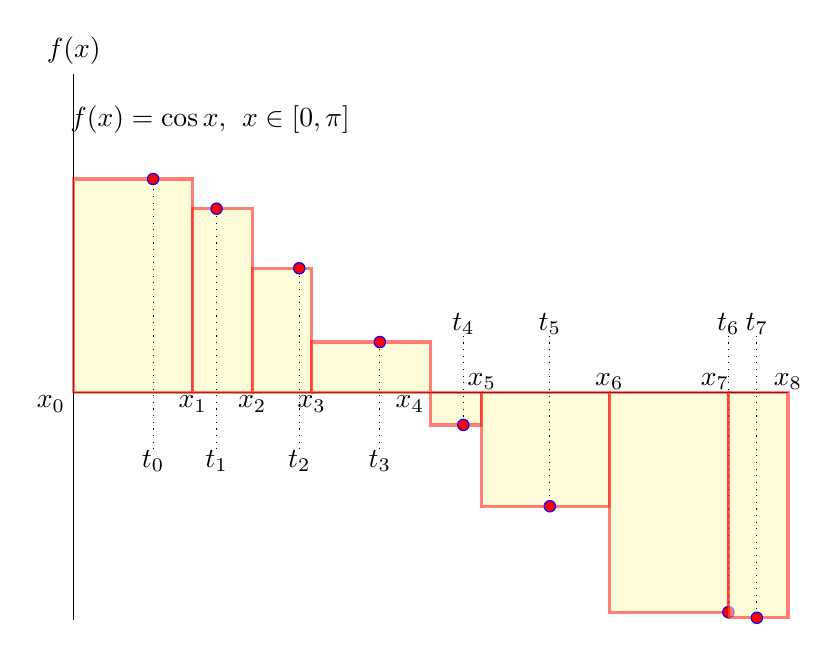
\begin{tikzpicture}[scale=\textwidth/4.2cm]
    % title and axes
    \node at (0.6, 1.2) {$f(x)=\cos x, \hspace{4pt} x \in [0, \pi]$};
    \draw (0, 0) -- (pi, 0);
    \draw (0, 0) -- (0, 1.4)
        node[above] {$f(x)$};
    \draw (0, 0) -- (0, -1);
    % graph
    \draw[black, very thick] plot[smooth] file {integrals_of_functions/python_generated_tables/cos_0_pi_riemann_sum.table};
    \draw[red, very thick, fill=yellow!30, opacity=0.5] (0, 0) 
        -- (pi/6, 0)
        -- (pi/6, {cos(pi/9 r)})
        -- (0, {cos(pi/9 r)})
        -- (0, 0);
    \node at (-0.1, -0.05) {$x_{0}$};
    \node at (pi/9, -0.3) {$t_{0}$};
    \node at (pi/6, -0.05) {$x_{1}$};
    \draw[black, dotted] (pi/9, -0.25) -- (pi/9, {cos(pi/9 r)});
    \draw[blue, fill=red] (pi/9, {cos(pi/9 r)}) circle (.25mm);
    \draw[red, very thick, fill=yellow!30, opacity=0.5] (pi/6, 0) 
        -- (pi/4, 0)
        -- (pi/4, {cos(pi/5 r)})
        -- (pi/6, {cos(pi/5 r)})
        -- (pi/6, 0);
    \node at (pi/5, -0.3) {$t_{1}$};
    \node at (pi/4, -0.05) {$x_{2}$};
    \draw[black, dotted] (pi/5, -0.25) -- (pi/5, {cos(pi/5 r)});
    \draw[blue, fill=red] (pi/5, {cos(pi/5 r)}) circle (.25mm);
    \draw[red, very thick, fill=yellow!30, opacity=0.5] (pi/4, 0) 
        -- (pi/3, 0)
        -- (pi/3, {cos(12*pi/38 r)})
        -- (pi/4, {cos(12*pi/38 r)})
        -- (pi/4, 0);
    \node at (12*pi/38, -0.3) {$t_{2}$};
    \node at (pi/3, -0.05) {$x_{3}$};
    \draw[black, dotted] (12*pi/38, -0.25) -- (12*pi/38, {cos(12*pi/38 r)});
    \draw[blue, fill=red] (12*pi/38, {cos(12*pi/38 r)}) circle (.25mm);
    \draw[red, very thick, fill=yellow!30, opacity=0.5] (pi/3, 0) 
        -- (pi/2, 0)
        -- (pi/2, {cos(12*pi/28 r)})
        -- (pi/3, {cos(12*pi/28 r)})
        -- (pi/3, 0);
    \node at (12*pi/28, -0.3) {$t_{3}$};
    \node at (8*pi/17, -0.05) {$x_{4}$};
    \draw[black, dotted] (12*pi/28, -0.25) -- (12*pi/28, {cos(12*pi/28 r)});
    \draw[blue, fill=red] (12*pi/28, {cos(12*pi/28 r)}) circle (.25mm);
    \draw[red, very thick, fill=yellow!30, opacity=0.5] (pi/2, 0) 
        -- (4*pi/7, 0)
        -- (4*pi/7, {cos(6*pi/11 r)})
        -- (pi/2, {cos(6*pi/11 r)})
        -- (pi/2, 0);
    \node at (6*pi/11, 0.3) {$t_{4}$};
    \node at (4*pi/7, 0.05) {$x_{5}$};
    \draw[black, dotted] (6*pi/11, 0.25) -- (6*pi/11, {cos(6*pi/11 r)});
    \draw[blue, fill=red] (6*pi/11, {cos(6*pi/11 r)}) circle (.25mm);
    \draw[red, very thick, fill=yellow!30, opacity=0.5] (4*pi/7, 0) 
        -- (3*pi/4, 0)
        -- (3*pi/4, {cos(2*pi/3 r)})
        -- (4*pi/7, {cos(2*pi/3 r)})
        -- (4*pi/7, 0);
    \node at (2*pi/3, 0.3) {$t_{5}$};
    \node at (3*pi/4, 0.05) {$x_{6}$};
    \draw[black, dotted] (2*pi/3, 0.25) -- (2*pi/3, {cos(2*pi/3 r)});
    \draw[blue, fill=red] (2*pi/3, {cos(2*pi/3 r)}) circle (.25mm);
    \draw[red, very thick, fill=yellow!30, opacity=0.5] (3*pi/4, 0) 
        -- (11*pi/12, 0)
        -- (11*pi/12, {cos(11*pi/12 r)})
        -- (3*pi/4, {cos(11*pi/12 r)})
        -- (3*pi/4, 0);
    \node at (11*pi/12, 0.3) {$t_{6}$};
    \node at (44*pi/49, 0.05) {$x_{7}$};
    \draw[black, dotted] (11*pi/12, 0.25) -- (11*pi/12, {cos(11*pi/12 r)});
    \draw[blue, fill=red] (11*pi/12, {cos(11*pi/12 r)}) circle (.25mm);
    \draw[red, very thick, fill=yellow!30, opacity=0.5] (11*pi/12, 0) 
        -- (pi, 0)
        -- (pi, {cos(22*pi/23 r)})
        -- (11*pi/12, {cos(22*pi/23 r)})
        -- (11*pi/12, 0);
    \node at (22*pi/23, 0.3) {$t_{7}$};
    \node at (pi, 0.05) {$x_{8}$};
    \draw[black, dotted] (22*pi/23, 0.25) -- (22*pi/23, {cos(22*pi/23 r)});
    \draw[blue, fill=red] (22*pi/23, {cos(22*pi/23 r)}) circle (.25mm);
\end{tikzpicture}
}
\begin{align*}
    &\text{The approximation can be computed with} \hspace{20pt} \sum_{i=0}^{7} f(t_{i})(x_{i+1} - x_{i})
\end{align*}
Taking a partition with uncountable infinitely many points between $0$ and $1$ is the key to computing the integral. The rectangles seen in this example each have an area: base times height. The difference $(x_{i+1} - x_{i})$ for each $i$ represent the bases, while the function value at $t_{i}$ for each $i$ represents the height. So, the integral of our function $f$ ---the value of which we will discuss shortly--- can be expressed as the limit 
\begin{align*}
    \lim_{n \longrightarrow \infty} \sum_{i=0}^{n-1} \cos(t_{i}) (x_{i+1} - x_{i}) = \sin x
\end{align*}
\end{example}

Most of the functions that we see in this course will be continuous, and integration on these continuous functions will more times than not require the use of antidifferentiation, as opposed to the computation of sums, on these continuous functions. 

\begin{example}
Take $f(x) = 1$. Let's say we want to take the integral of $f$. The question you should ask yourself is:
\begin{align*}
    &\text{The derivative of which function is equal to} \hspace{4pt} 1?\\[2ex]
    &\text{Meaning, what is $g$, when} \hspace{4pt} \dfrac{d}{dx}g(x) = 1
\end{align*}
Because we already learned
\begin{align*}
    \dfrac{d}{dx} (x+c) = \dfrac{d}{dx} x + \dfrac{d}{dx} c = 1 + 0 = 1 \hspace{20pt} \text{where} \hspace{4pt} c \in \mathbb{R}
\end{align*}
we have that $g(x) = x+c$ and 
\begin{align*}
    g(x) = \int_{} 1 dx = x + c
\end{align*}
which we could represent without the $1$ under the integral sign as 
\begin{align*}
    g(x) = \int_{} dx = x+c
\end{align*}
\end{example}